\documentclass[9pt, xcolor=table]{beamer}

\usepackage[utf8]{inputenc}
\usepackage[round, comma]{natbib}
\usepackage{amsmath}
\usepackage{hyperref}
\usepackage{amsfonts}
\usepackage{verbatim}
\DeclareMathOperator*{\argmin}{arg\,min}



\mode<presentation> {

\usetheme{Madrid}

\setbeamertemplate{navigation symbols}{} 
\useinnertheme{circles}
\definecolor{greenish}{RGB}{0, 153, 76}
\usecolortheme[named=greenish]{structure}
}

\setbeamertemplate{headline}
{%
  \begin{beamercolorbox}[ht=3.5ex,dp=1.125ex,%
      leftskip=.3cm,rightskip=.3cm plus1fil]{section in head/foot}
    \usebeamerfont{section in head/foot}\usebeamercolor[fg]{section in head/foot}%
\insertsectionnavigationhorizontal{\paperwidth}{\hskip0pt plus1fill}{\hskip0pt plus1fill}
  \end{beamercolorbox}%
  \begin{beamercolorbox}[colsep=1.5pt]{middle separation line head}
  \end{beamercolorbox}
  \begin{beamercolorbox}[colsep=1.5pt]{lower separation line head}
  \end{beamercolorbox}
}

\title[Interpretation of black box models]{Interpretation of black box models using tree-based surrogate models \newline \small{Simulations}}
\author[Sofia Loibl]{Sofia Loibl}
\institute[LMU]{LMU München}
\date{\today}

\begin{document}

\begin{frame}
\titlepage 
\end{frame}


\section{Selection Bias}
\begin{frame}{Selection Bias}
\textbf{Goal:} 

Comparison of different versions of SLIM, MOB, CTree and GUIDE with respect to selection bias
\vspace{0.5cm}


\textbf{Selection bias:} 

An algorithm for recursive partitionig is called unbiased when, under the conditions of the null hypothesis of independence between a response $Y$ an covariates $X_{1},...X_{m}$ the probability of selecting covariate $X_{j}$ is $1/m$ for all $j = 1,...,m$ regardless of the measurement scales of number of missing values. \citep{Hothorn.2006}
\vspace{0.5cm}

\textbf{Simulation Setting:} $1000$ simulation runs with $n= 1000$
\end{frame}


\begin{frame}{Scenario Independence}
$X_{1}, X_{2} \sim U(0,1)$; 
$X_{3} \sim U(0,1)$ and rounded to one digit;
$X_{4}$ binary;
$X_{5}$ categorical with 5 levels;
$X_{6}$ categorical with 8 levels\\
$Y \sim N(0,1)$

\begin{figure}
    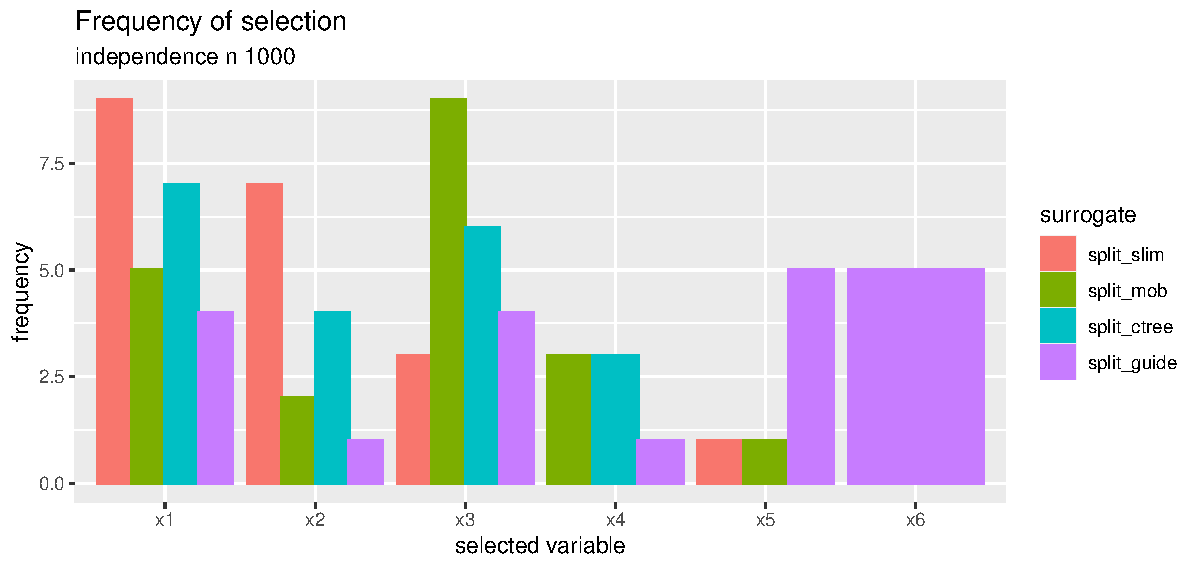
\includegraphics[width=11cm]{Figures/simulations/batchtools/selection_bias_results/independence_n1000.pdf}
\end{figure}
\end{frame}


\begin{frame}{Scenario Independence small}
All $X_j \sim U(0,1)$; $X_3$ rounded to one digit, $X_4$ rounded to two digits\\
$Y \sim N(0,1)$
\begin{figure}
    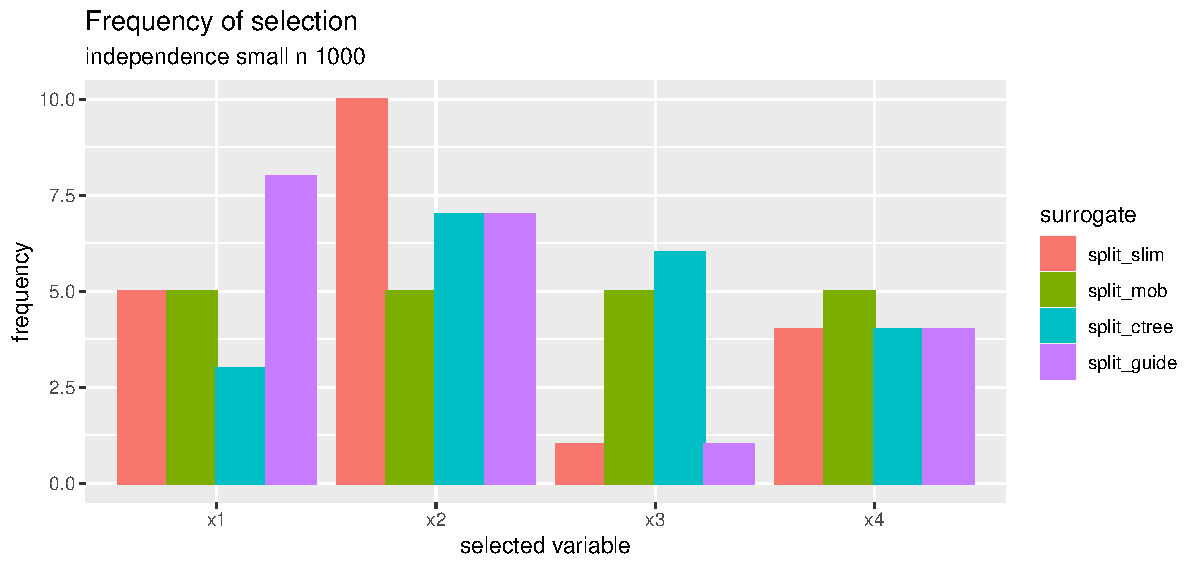
\includegraphics[width=11cm]{Figures/simulations/batchtools/selection_bias_results/independence_small_n1000.pdf}
\end{figure}

\end{frame}

\begin{frame}{Scenario Interaction}

All $X_j \sim U(0,1)$; $X_3$ rounded to one digit, $X_4$ rounded to two digits\\
$Y = X_1 + X_2 + X_3 + X_4 + X_1 X_2 + X_1 X_3 + X_1 X_4 + X_2 X_3 + X_2 X_4 + X_3 X_4 + eps$
\begin{figure}
    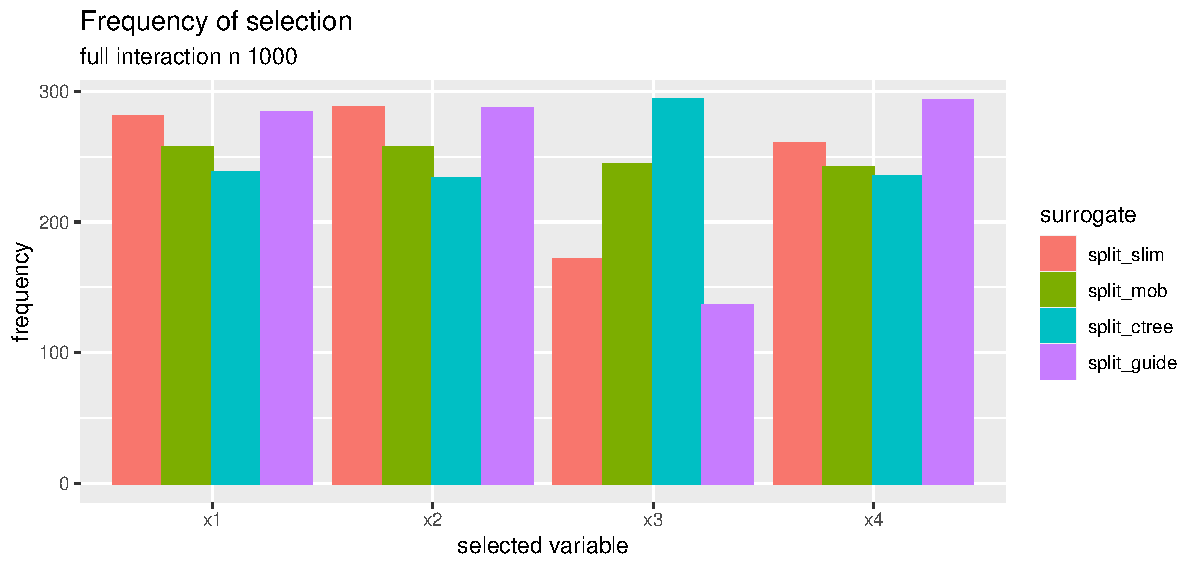
\includegraphics[width=11cm]{Figures/simulations/batchtools/selection_bias_results/full_interaction_n1000.pdf}
\end{figure}
\end{frame}



\end{document}